\chapter{Implementación}
En el siguiente capítulo se describe la implementación del sistema desarrollado durante la memoria. Se implementaron dos posibles arquitecturas para un sistema de reconocimiento de videos. La primera alternativa graba videos con el dispositivo móvil y los envía completos al servidor, para que este calcule sus descriptores y realice la búsqueda, llamamos a esta la alternativa \emph{centralizada} pues todos los cálculos son realizados en el servidor. La segunda alternativa del sistema realiza los cálculos de descriptores en el mismo dispositivo móvil que graba el video, luego solo es necesario enviar los descriptores calculados al servidor que ejecuta la búsqueda, llamamos a esta alternativa \emph{distribuida} pues los cálculos están repartidos entre el cliente y el servidor.

El capítulo se divide en una sección para la alternativa centralizada y otra para la distribuida. A su vez cada sección se divide en la implementación del cliente Android y el servidor.
\TODO{Pensar en mejores nombres para los sistemas alternativos}


\section{Sistema Centralizado}

La figura~\ref{arquitectura_centralizada} muestra la arquitectura de la versión centralizada del sistema. En esta versión el dispositivo móvil es usado solo para grabar un video corto. El archivo de video resultante es enviado al servidor (1), el cual calcula sus descriptores (2) y realiza la búsqueda en la base de datos (3) , devolviendo los resultados al cliente (4).
A continuación se detalla la implementación de esta versión del sistema, separando el cliente Android del servidor.
	\begin{figure}[!h]
		\centering
		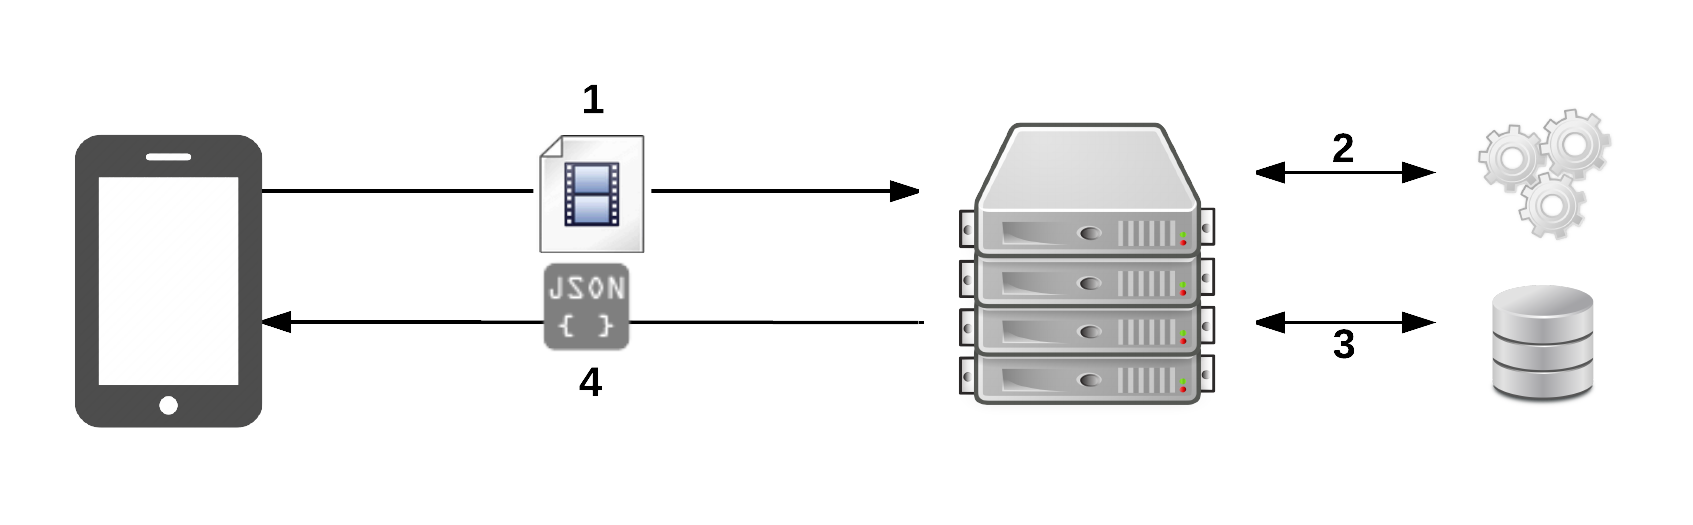
\includegraphics[scale=1]{imagenes/cap3/arquitectura_centralizada}
		\caption{Diagrama de la arquitectura del sistema centralizado.}
		\label{arquitectura_centralizada}
	\end{figure}
\subsection{Cliente Android}
En esta versión el cliente Android es responsable de grabar un video usando la cámara del dispositivo, enviarlo al servidor y de mostrarle al usuario los resultados de la búsqueda realizada por el servidor. Para cada una de estas responsabilidades se implementó un módulo.

\subsubsection*{Grabación}

El módulo de grabación es responsable de grabar un video usando la cámara del dispositivo y guardar el archivo resultante. Para lograr esto se creó el fragmento \texttt{VideoRecordFragment}, esta clase presenta al usuario un breve mensaje de instrucciones y un botón para comenzar la grabación. La figura ~\ref{pantalla_video_record_fragment} corresponde a la pantalla que ve el usuario al iniciar la aplicación. Al hacer click en el botón \emph{grabar} el sistema invoca a la aplicación por defecto de grabación de videos de Android por medio de un Intent.
La aplicación de grabación presenta un preview de la cámara como muestra la figura~\ref{pantalla_video_record_android}, en este momento el usuario debe iniciar la grabación, que dura por un máximo de 5 segundos y guarda en un archivo el video resultante. Después de terminar la grabación el sistema le cede de vuelta el control a la aplicación, con esto se procede a enviar el video resultante al servidor.
\TODO{insertar aquí pantallazos de la aplicación}

\subsubsection*{Conexión con el servidor}
El módulo de conexión con el servidor es responsable de enviar al servidor el video capturado por el módulo anterior. Se implementó la clase \texttt{FromVideoSearchRequest} que recibe un archivo y ejecuta un petición HTTP Post al servidor, eviando el archivo grabado y un parámetro con el tipo de descriptor para usar en la búsqueda.  Una vez se termina el envío de datos al servidor se cambia la interfaz por una pantalla inicialmente vacía donde se mostraran los resultados. 

\subsection{Servidor}

\section{Sistema Distribuido}

La figura~\ref{arquitectura_distribuida} ilustra la arquitectura de esta versión del sistema. El cálculo de descriptores para la búsqueda es realizado por el cliente Android (1) utilizando las herramientas para computación paralela descritas en secciones anteriores. Una vez calculados, se envían solo estos descriptores al servidor (2) el cual los usa para realizar la búsqueda por similitud (3) y luego comunica los resultados de vuelta al cliente (4).

	\begin{figure}[!h]
		\centering
		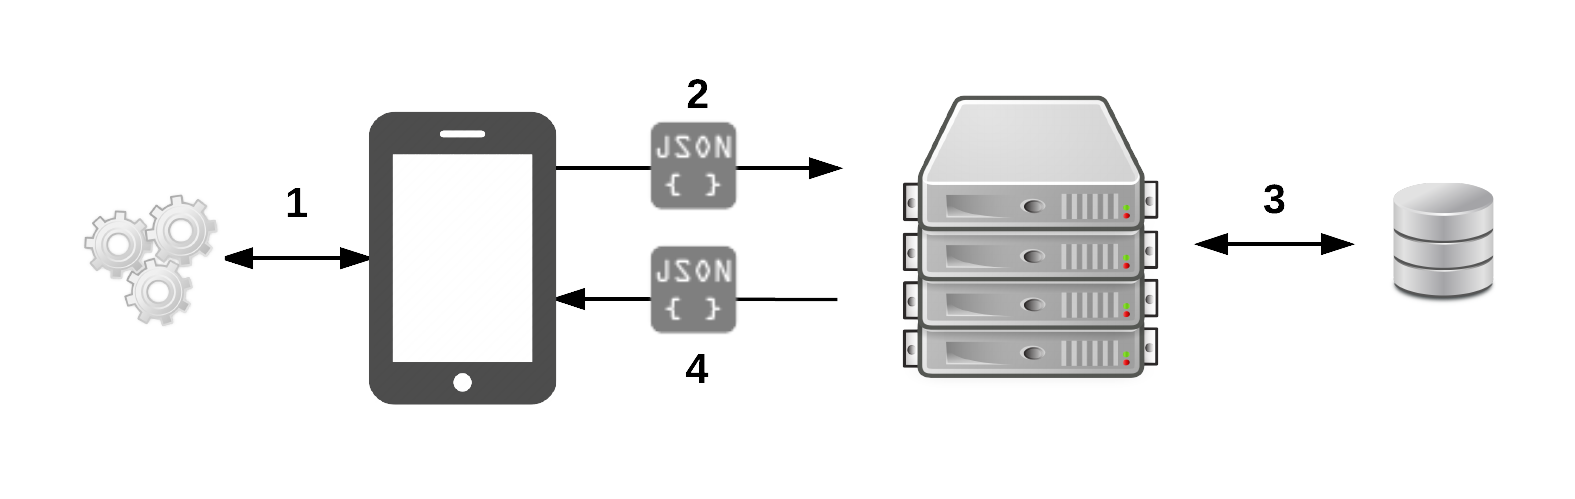
\includegraphics[scale=1]{imagenes/cap3/arquitectura_distribuida.png}
		\caption{Diagrama de la arquitectura del sistema distribuido.}
		\label{arquitectura_distribuida}
	\end{figure}

A continuación se detalla la implementación de tanto el cliente Android como el servidor y se comentan las diferencias con respecto a la versión descrita anteriormente.

\subsection{Cliente Android}
\subsection{Servidor}
